\part{Second-Order-DEs}
\lecture{Second Order DEs}{Second-Order-DEs}
\section{Second Order DEs}

\title{Ordinary Differential Equations}
\subtitle{Math 232 - Linear, Constant Coefficient ODEs}
\date{8 Oct 2012}

\begin{frame}
  \titlepage
\end{frame}

\begin{frame}
  \frametitle{Outline}
  \tableofcontents[pausesection,hideothersubsections]
\end{frame}


\subsection{Second Order DEs}


\iftoggle{clicker}{%
\begin{frame}
  \frametitle{Clicker Quiz}

      \ifnum\value{clickerQuiz}=1{%

        \vfill

        Are the vectors $\vecTwo{-1}{1}$ and $\vecTwo{2}{-2}$ linearly independent?

        \vfill

        \begin{tabular}{ll}
          A: & Yes \\
          B: & No
        \end{tabular}


        \vfill

      }\fi

      \ifnum\value{clickerQuiz}=2{%

        \vfill

        Are the vectors $\vecTwo{1}{1}$ and $\vecTwo{3}{2}$ linearly independent?

        \vfill

        \begin{tabular}{ll}
          A: & Yes \\
          B: & No
        \end{tabular}

        \vfill

     }\fi
   
     \ifnum\value{clickerQuiz}=3{%

        \vfill

    }\fi
  

\end{frame}
}



\begin{frame}
  \frametitle{Second Order Equations}

  The General, Constant Coefficient, Linear, Second Order Homogeneous
  Differential Equation:
  \begin{eqnarray*}
    {\color{red}m} x'' + {\color{red}b} x' + {\color{red}k}x & = & 0.
  \end{eqnarray*}
  The parameters {\color{red}$m$}, {\color{red}$b$}, and {\color{red}$k$} are constants.

  This is also called the ``Damped Harmonic Oscillator.''

\end{frame}

\subsection{Horizontal Spring/Mass Systems}

\begin{frame}
  \frametitle{Horizontal Spring/Mass System}

  \only<1>{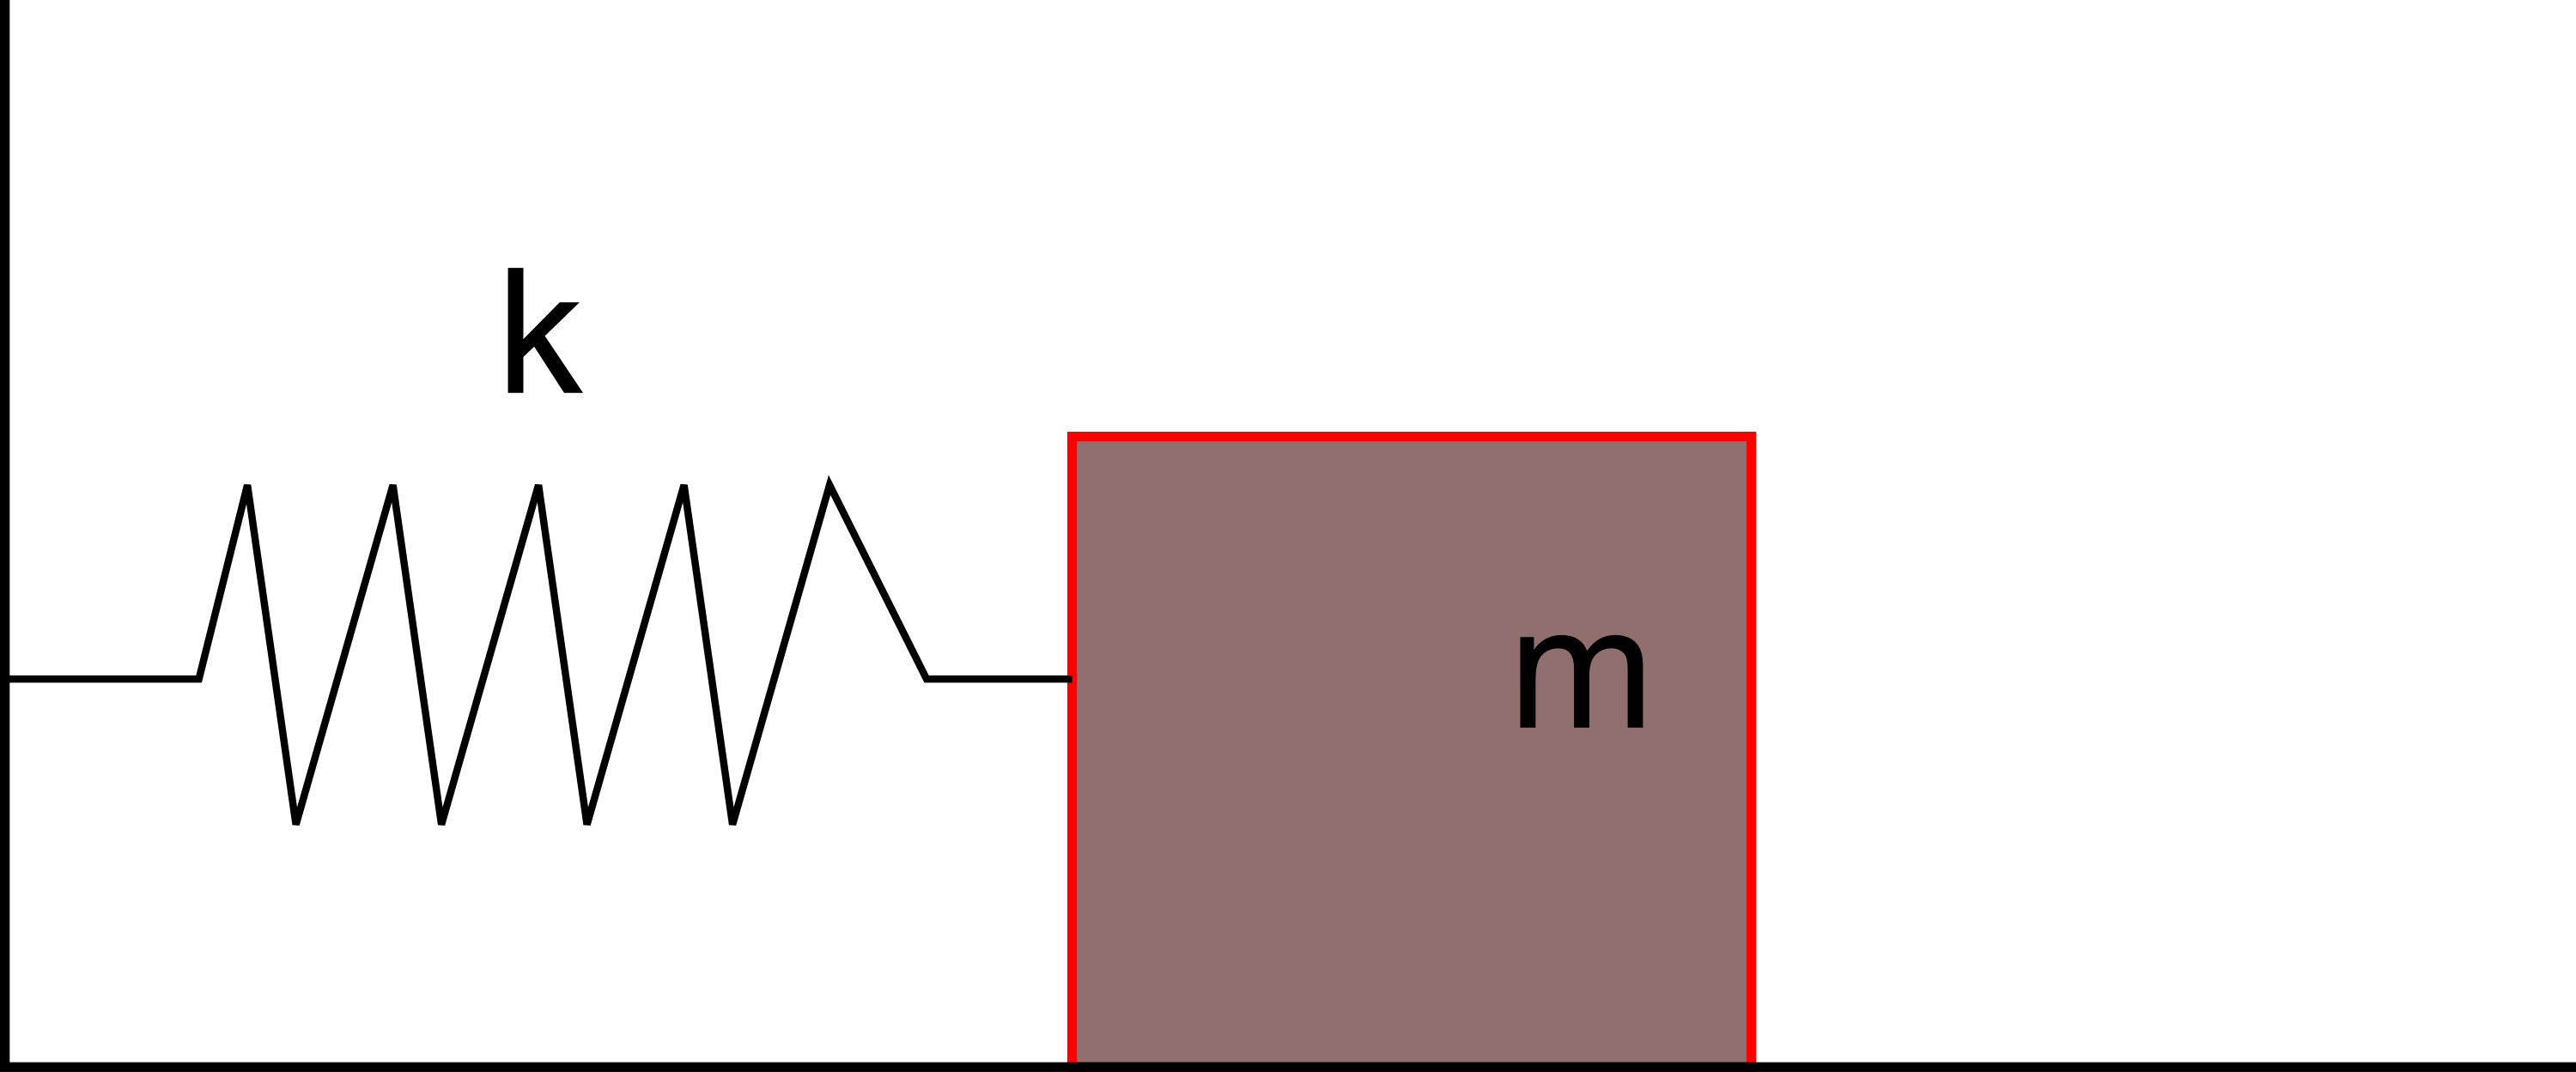
\includegraphics[width=6cm]{img/springMassStatic}}
  \only<2>{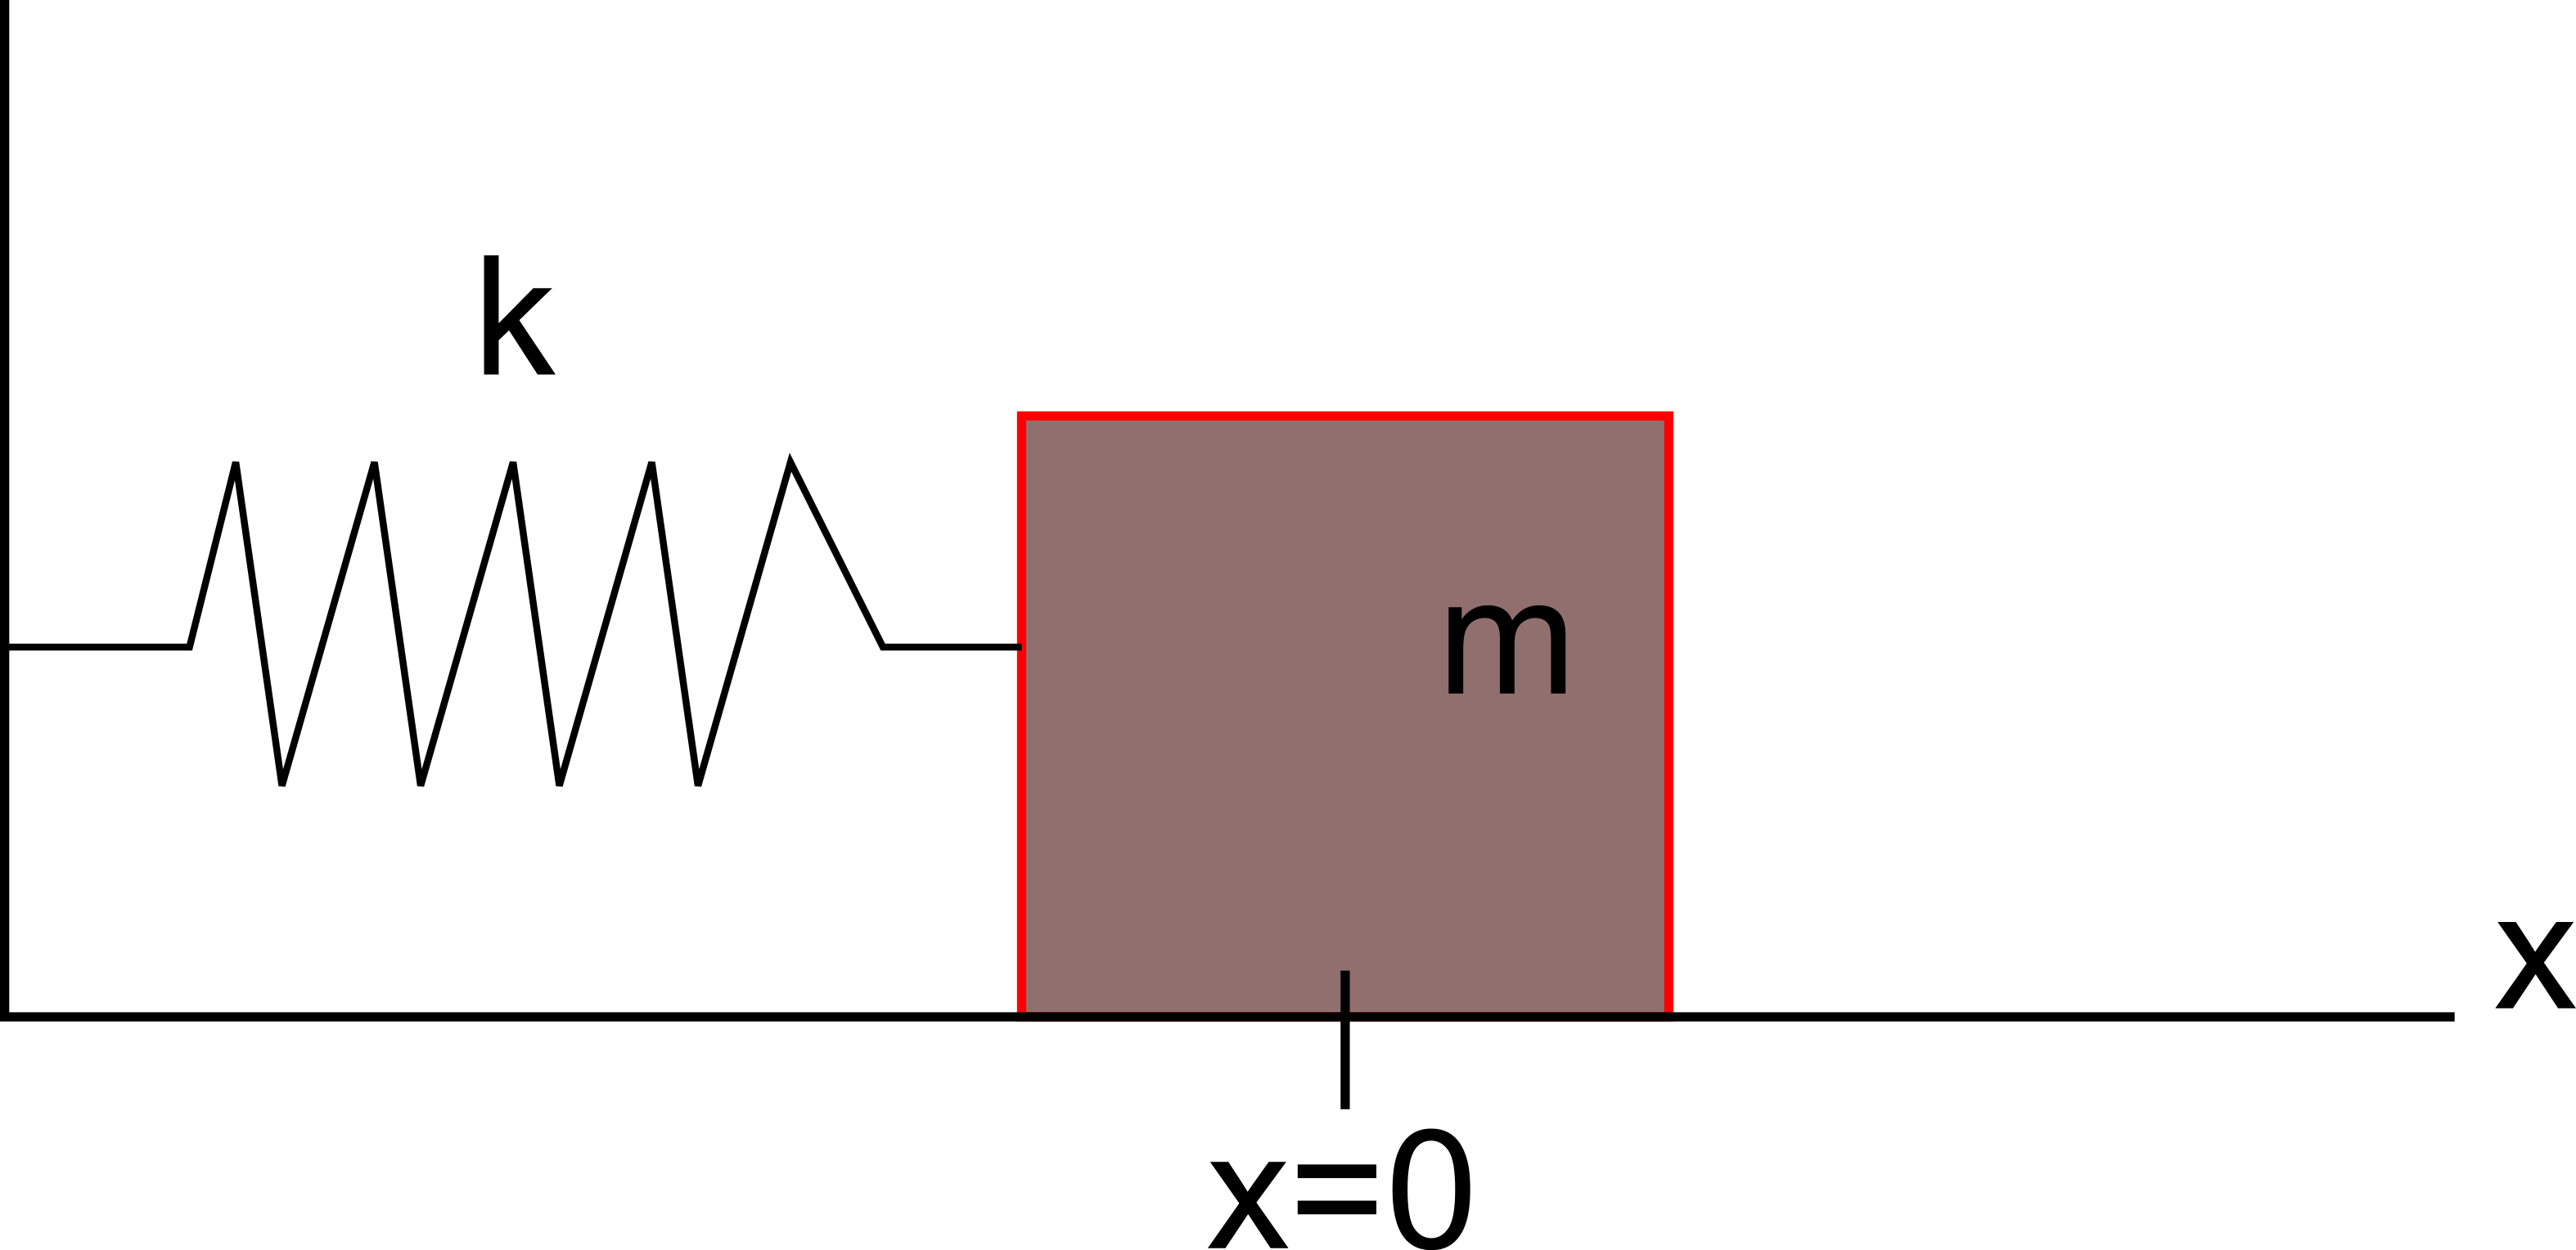
\includegraphics[width=6cm]{img/springMassStaticCoordinates}}
  \only<3>{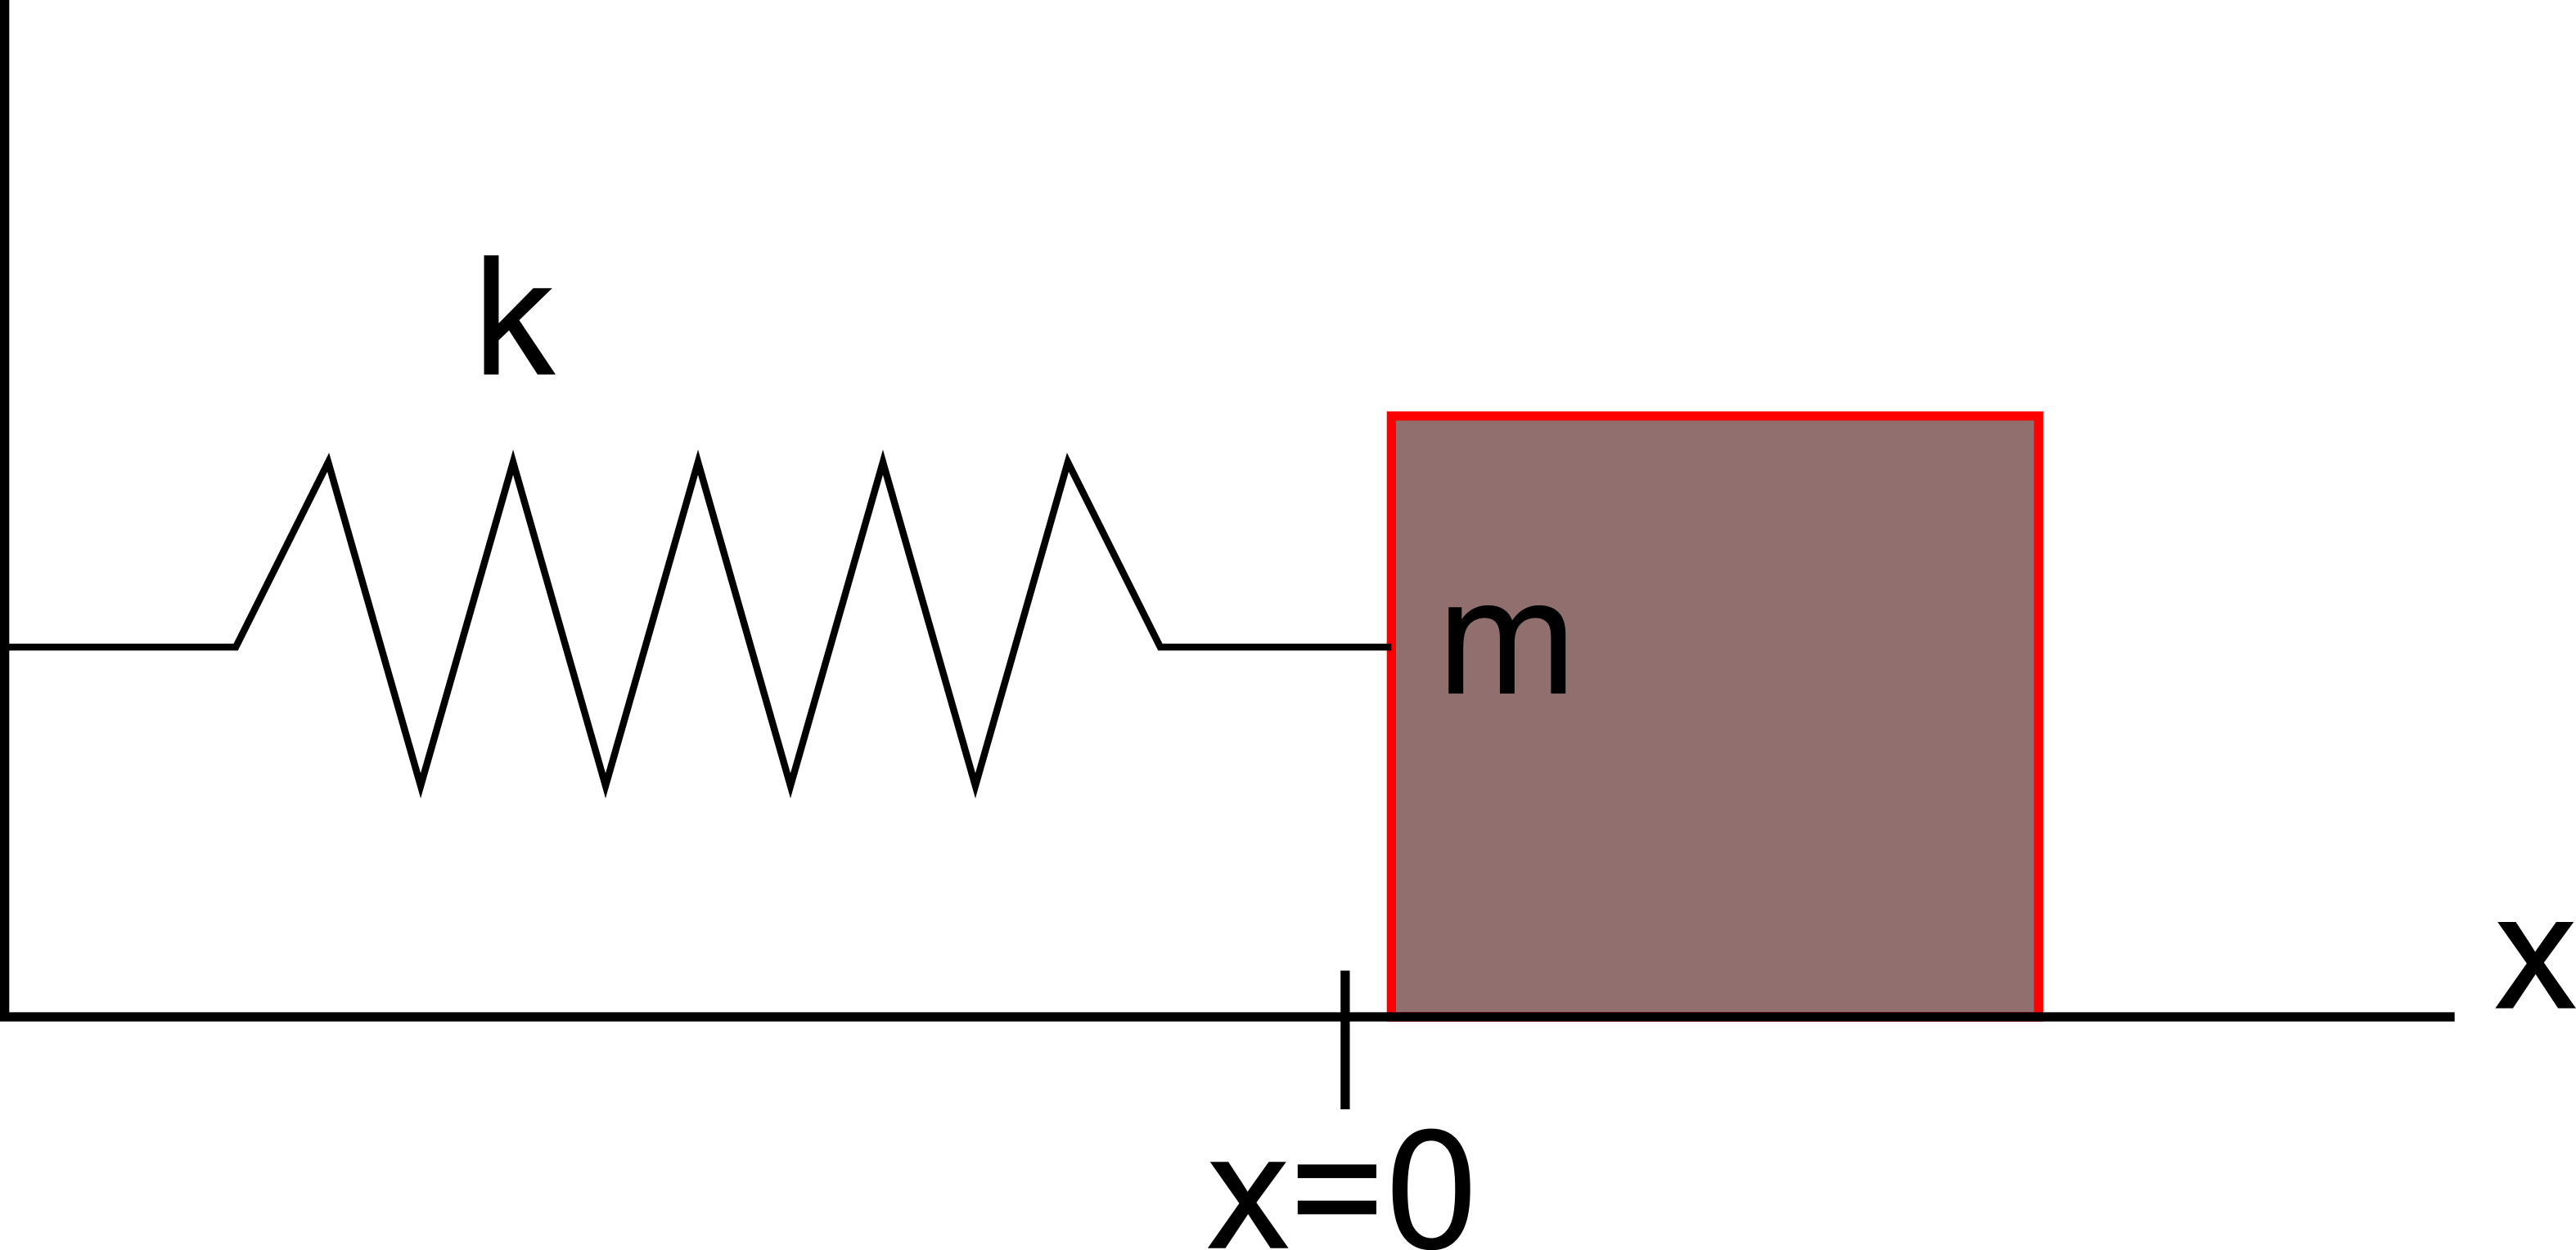
\includegraphics[width=6cm]{img/springMassDynamic}}
  \only<4->{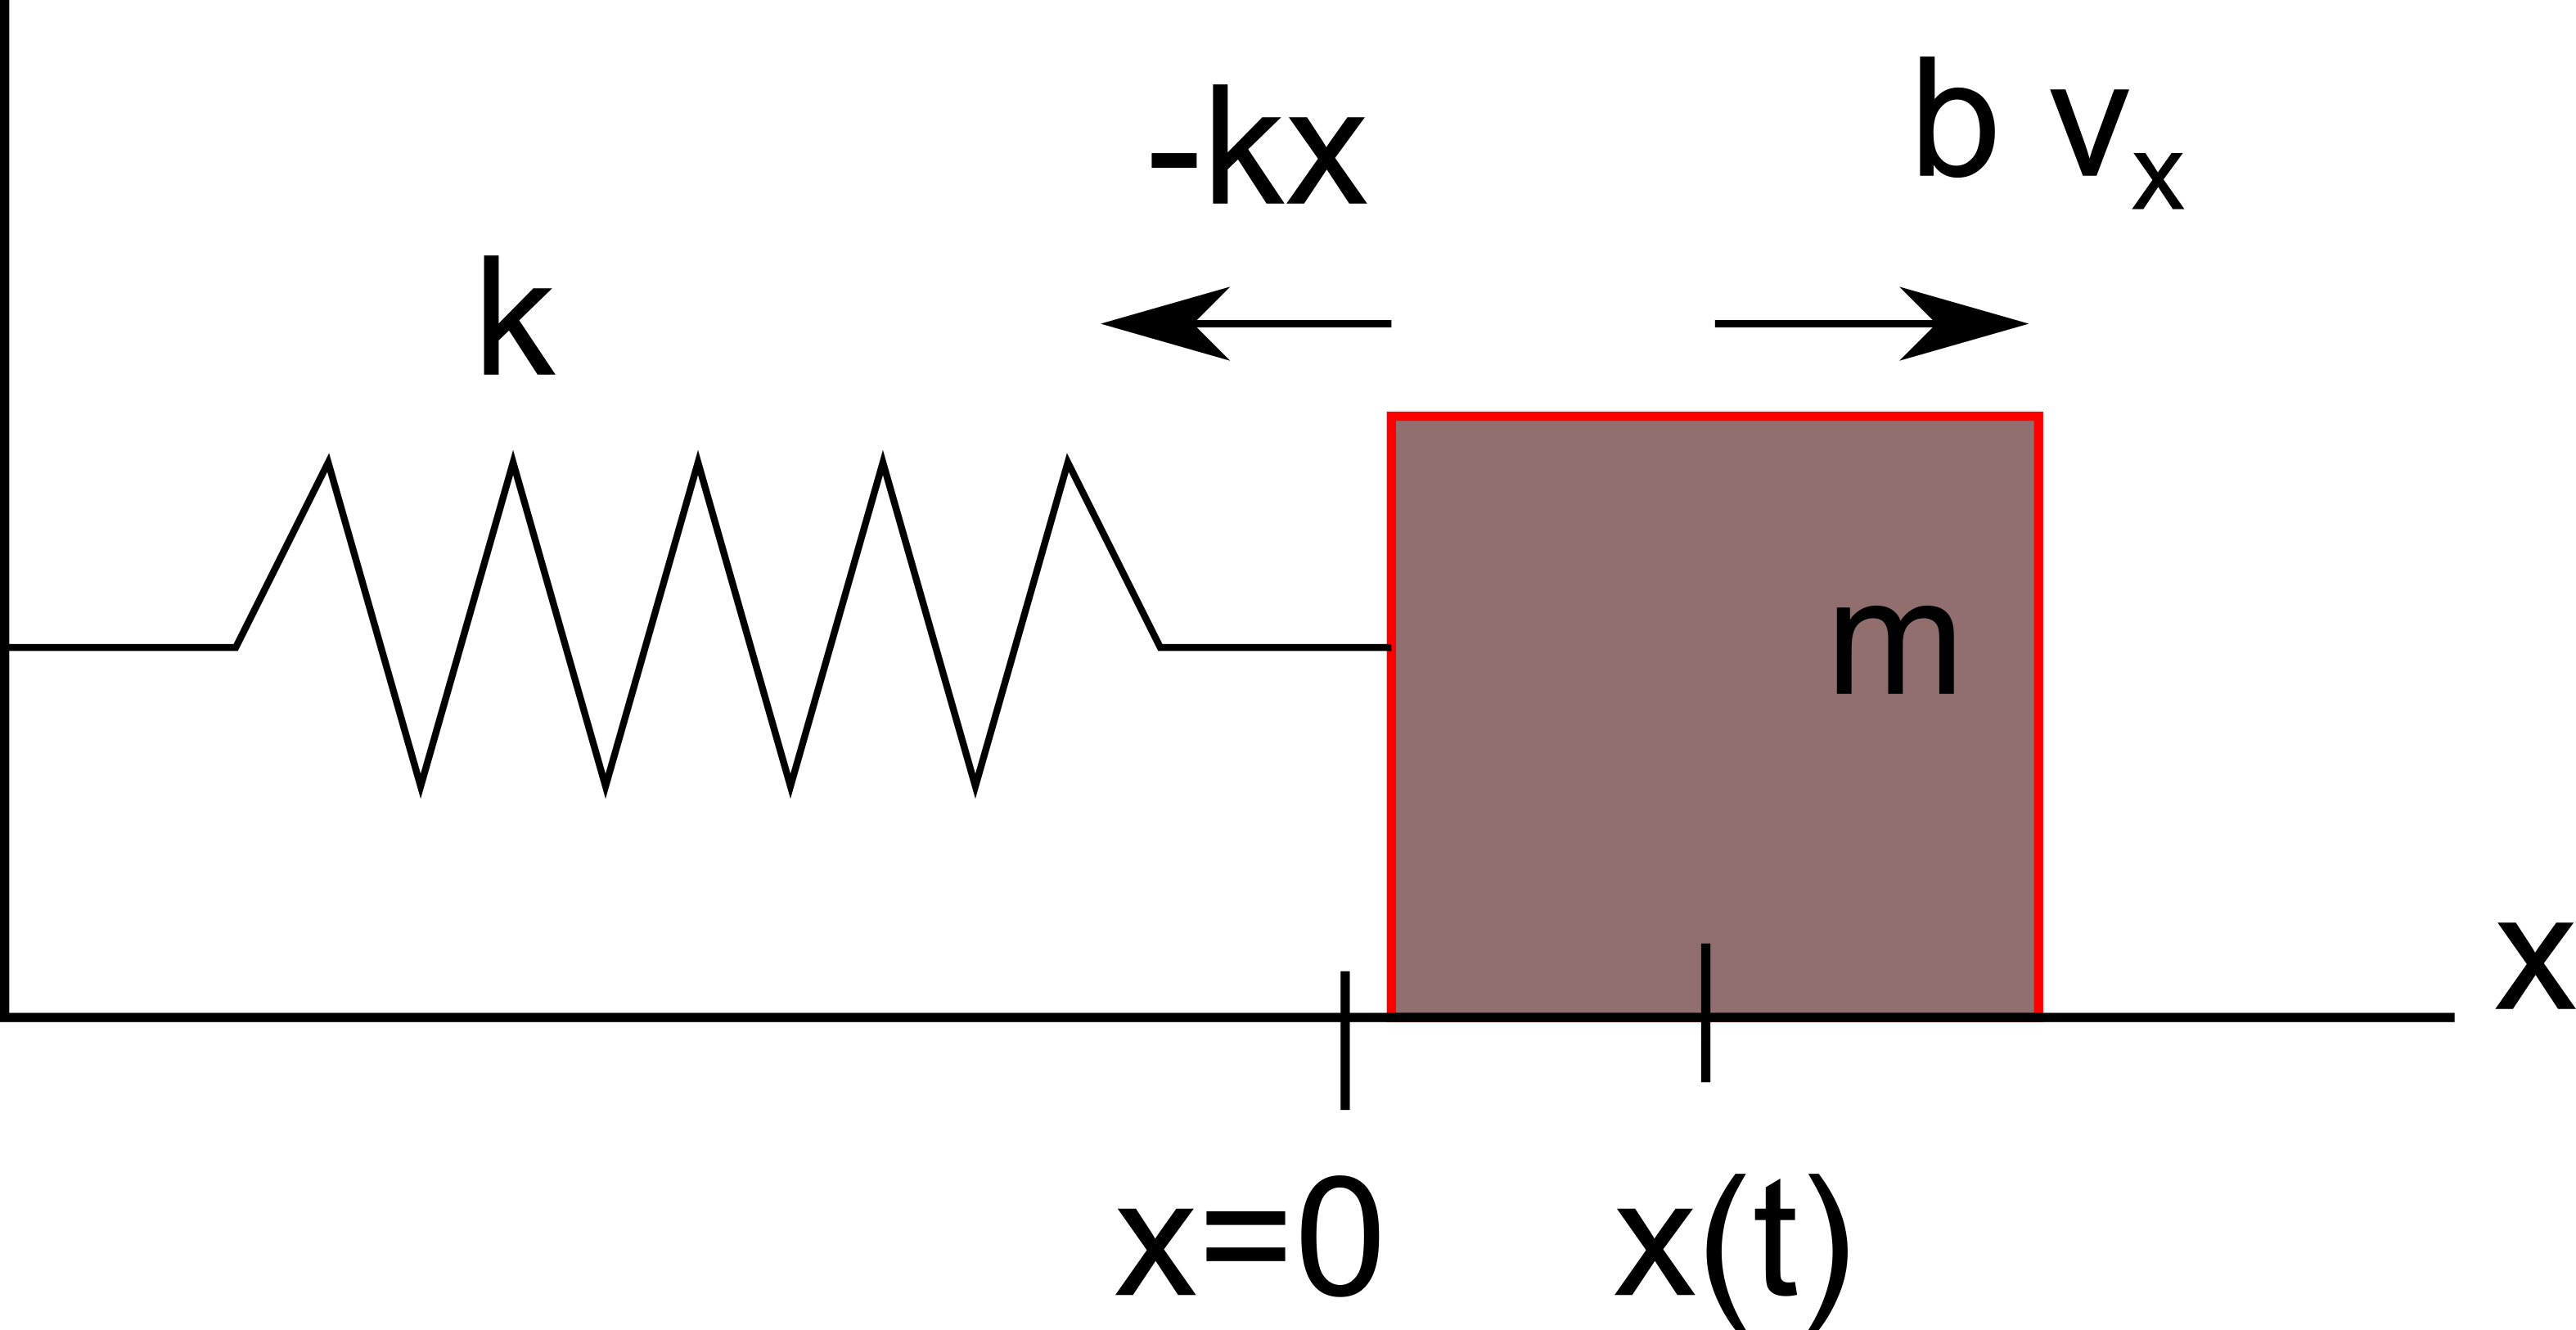
\includegraphics[width=6cm]{img/springMassDynamicVectors}}

  \uncover<4->{%
    Newton's Second Law:
    \begin{eqnarray*}
      \frac{d}{dt} \lp m \vec{v} \rp & = & \sum_i \vec{F}_i \\
      & = & -kx - bv_x 
    \end{eqnarray*}
    or
    \begin{eqnarray*}
      mx'' + bx' + kx & = & 0.
    \end{eqnarray*}

    If $b=0$ it is an ``\textbf{undamped''} system, otherwise it is ``\textbf{damped}.''
  }

\end{frame}


\begin{frame}
  \frametitle{Example}

  A mass of 2 kg is resting on an horizontal table and attached to a
  linear spring which has a spring constant of 3 N/m. The force of
  friction is 1.5 times the velocity. The block is pulled to the left
  0.5m and let go. Find the governing equation.

  \uncover<2->
  {
    \begin{eqnarray*}
      2 x'' + 1.5 x' + 3x & = & 0, \\
      x(0) & = & -.5m, \\
      x'(0) & = & 0 m/s.
    \end{eqnarray*}

    Need two initial conditions!
  }

\end{frame}


\begin{frame}
  \frametitle{Lots of variations}

  \begin{itemize}
  \item Could say that the spring stretched .25 m when 2N is applied.
  \item Could say that the force of friction is 0.5N when it is moving
    .3 m/s. 
  \end{itemize}

  See example on p. 197.

\end{frame}

\subsection{Undamped Systems}


\begin{frame}
  \frametitle{Special Case}

  No friction, $b=0$: \textit{(Use your intuition!)} 
  \begin{eqnarray*}
    m x'' + kx & = & 0.
  \end{eqnarray*}

  \uncover<2->
  {
    Assume solutions of the form 
    \begin{eqnarray*}
      x & = & C_1 \cos(\omega t) + C_2 \sin(\omega t) \\
      \uncover<3->
      {
        x' & = & -\omega C_1 \sin(\omega t) + \omega C_2 \cos(\omega t) \\
      }
      \uncover<4->
      {
        x'' & = & -\omega^2 C_1 \cos(\omega t) - \omega^2 C_2 \sin(\omega t) \\
      }
    \end{eqnarray*}
  }

\end{frame}


\iftoggle{clicker}{%
\begin{frame}
  \frametitle{Clicker Quiz}

      \ifnum\value{clickerQuiz}=1{%

        \vfill

        Suppose that the spring/mass system has no friction,
        $b=0$, 
        \begin{eqnarray*}
          m x'' + kx & = & 0.
        \end{eqnarray*}        
        What kind of behavior do you expect?

        \vfill

        \begin{tabular}{ll}
          A: & Infinite, perfect oscillations until the end of time. \\
             & (or the end of today's class whichever comes first)  \\
          B: & Oscillations slowly dieing out.  \\
          C: & Oscillations with slow but steady decay \\
          D  & Oscillations with exponential decay
        \end{tabular}


        \vfill

      }\fi

      \ifnum\value{clickerQuiz}=2{%

        \vfill
        Suppose that the spring/mass system has no friction,
        $b=0$, 
        \begin{eqnarray*}
          m x'' + kx & = & 0.
        \end{eqnarray*}        
        What kind of behavior do you expect?

        \vfill

        \begin{tabular}{ll}
          A: & Infinite, perfect oscillations until the end of time. \\
             & (or the end of today's class whichever comes first)  \\
          B: & Oscillations slowly dieing out.  \\
          C: & Oscillations with slow but steady decay \\
          D  & Oscillations with exponential decay
        \end{tabular}


        \vfill

     }\fi
   
     \ifnum\value{clickerQuiz}=3{%

        \vfill

    }\fi
  

\end{frame}
}


\begin{frame}
  \frametitle{Special Case}

  No friction, $b=0$:
  \begin{eqnarray*}
    m x'' + kx & = & 0.
  \end{eqnarray*}

  \uncover<2->
  {
    \begin{eqnarray*}
      0 & = & mx''+kx \\
        & = & - m\omega^2 C_1 \cos(\omega t) - m\omega^2 C_2 \sin(\omega t) \\
        &   & + k C_1 \cos(\omega t) + k C_2 \sin(\omega t)\\
        & = & \lp -m \omega^2 + k \rp C_1 \cos(\omega t) +
              \lp -m \omega^2 + k \rp C_2 \sin(\omega t)
    \end{eqnarray*}
  }

  \uncover<3->
  {
    \begin{eqnarray*}
      \Rightarrow \omega & = & \pm \sqrt{\frac{k}{m}}.
    \end{eqnarray*}
  }

  \vfill

\end{frame}


\begin{frame}
  \frametitle{Special Case}

  No friction, $b=0$:
  \begin{eqnarray*}
    m x'' + kx & = & 0.
  \end{eqnarray*}

  \begin{eqnarray*}
    x & = & C_1 \cos\lp\sqrt{\frac{k}{m}} t\rp +
    C_2 \sin\lp\sqrt{\frac{k}{m}} t\rp \\
    & = & A \cos\lp \sqrt{\frac{k}{m}} t - \delta \rp.
  \end{eqnarray*}

  Period = T,
  \begin{eqnarray*}
    \sqrt{\frac{k}{m}} T & = & 2\pi, \\
    \Rightarrow T & = & 2 \pi \sqrt{\frac{m}{k}}.
  \end{eqnarray*}

\end{frame}


\begin{frame}
  \frametitle{Example}

  An horizontal spring/mass system is to be constructed using a 2 kg
  mass. What spring constant should be used so that it oscillates at 3
  oscillations per second?

  \begin{eqnarray*}
    2 x'' + kx & = & 0 \\
    x & = & A \cos\lp \sqrt{\frac{k}{2}} t - \delta \rp \\
  \end{eqnarray*}

  \uncover<2->
  {
    3 oscillations per second means that
    \begin{eqnarray*}
      \sqrt{\frac{k}{2}} \lp \frac{1}{3} \rp & = & 2 \pi, \\
      k & = & 72 \pi^2.
    \end{eqnarray*}
  }

\end{frame}

\subsection{RCL Circuits}

\begin{frame}
  \frametitle{RCL Circuit}

  See pp. 202-204 for more information about RCL circuits.

  Voltage drops: \\
  \begin{tabular}{l@{~$=$~}l}
    Resistor & $RI$ \\
    Inductor & $LI'$ \\
    Capacitor & $\frac{Q}{C}$.
  \end{tabular}

  \begin{eqnarray*}
    L I' + RI + Q/C & = & v(t) \\
    L Q'' + RQ' + Q'/C & = & v(t).
  \end{eqnarray*}

\end{frame}



% LocalWords:  Clarkson pausesection hideothersubsections DEs ODEs undamped kx
% LocalWords:  mx RCL
